\subsection{Class Diagram}



%Describe here the class diagram of your project

The class diagram for our recipe sharing platform outlines the essential entities and their relationships, defining user interaction and navigation within the platform.

\begin{figure}[h]
    \centering
    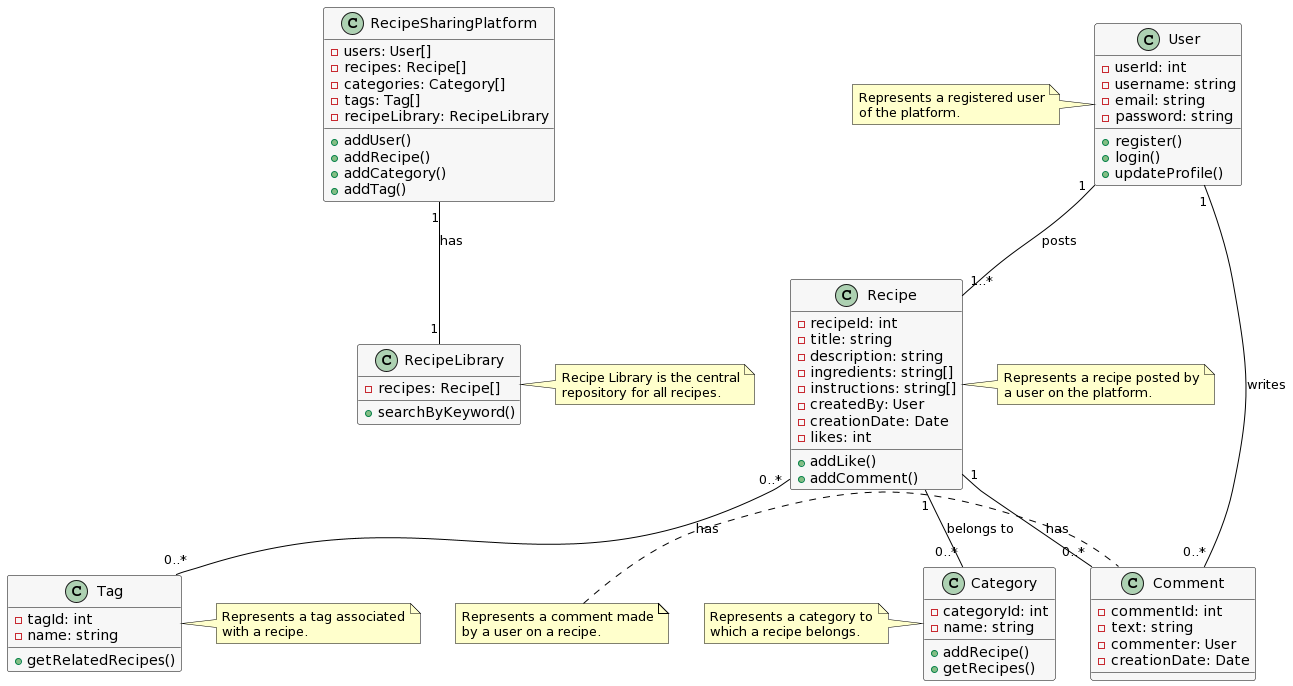
\includegraphics[width=0.75\linewidth]{sections/BLL/Class_diagram_Boats.png}
    \caption{Class Diagram for Recipe Platform}
    \label{fig:class_diagramRP}
\end{figure}


The \textbf{User class} serves as the foundation of the recipe sharing platform, representing individuals who actively participate within the system. Each user is uniquely identified by a userId and maintains essential credentials such as username, email, and password, crucial for user authentication and identification purposes. Users utilize these attributes to register, log in, and personalize their profiles, enhancing their engagement with the platform. For instance, a user with the username "foodie123" will always be interacting on the platform with the userId after it registers using the email "foodie@example.com" and a chosen password to access platform features. Recipes, the main content of the platform, are contained within the \textbf{Recipe class}. Each recipe instance is distinguished by a recipeId, a descriptive title, a summary of the dish, a list of ingredients, detailed preparation instructions, the creator's identity, creation date, and the number of likes received. Users interact with recipes by expressing appreciation through likes or contributing comments to share insights or recommendations. For instance, "ChefJane" might share her renowned "Spaghetti Carbonara" recipe, detailing ingredients and preparation steps.
Comments on recipes are managed by the \textbf{Comment class}, which includes a commentId, the textual content, the commenter's identity, and the submission date. Comments foster user interaction, allowing for discussions, feedback, or queries related to specific recipes.
Recipes are further categorized using the \textbf{Category class}, which assigns a categoryId and a descriptive name to group recipes based on themes, cuisines, or dietary preferences, enhancing organization and navigation. For example, recipes like "Grilled Salmon" or "Miso Soup" may belong to categories like "Seafood" or "Japanese Cuisine."
Tags, represented by the \textbf{Tag class}, serve as descriptive labels associated with recipes, aiding in search and categorization. Each tag is identified by a tagId and a descriptive name, enabling users to discover recipes based on specific ingredients or attributes.
The \textbf{RecipeLibrary class} acts as the central repository for all recipes, managing an array of Recipe objects and providing search functionality for users to explore culinary content easily. Aside from this, the \textbf{RecipeSharingPlatform class} defines platform functionality, overseeing user management, recipe sharing, category and tag administration, and recipe discovery. Users interact with the platform through various actions such as account registration, recipe sharing, category exploration, and community engagement via comments and likes.

